% ==========================================
% BAB IV DESAIN KONSEP SOLUSI
% ==========================================
\chapter{DESAIN KONSEP SOLUSI}
\label{chap:desain-konsep-solusi}

Bab ini menyajikan desain konsep sistem rangkuman otomatis berbasis AI yang diusulkan sebagai solusi untuk mengatasi masalah \textit{information overload} di komunitas Telegram Michael Yeoh. Desain konsep divisualisasikan melalui model arsitektural yang membandingkan sistem saat ini dengan sistem yang diusulkan, diikuti dengan penjelasan komprehensif tentang komponen-komponen utama, aliran data, dan perbedaan fundamental dengan kondisi \textit{existing}.

% ==========================================
\section{Perbandingan Sistem Saat Ini dengan Sistem yang Diusulkan}
\label{sec:before-after-comparison}

\subsection{Model Konseptual Sistem Saat Ini (\textit{Before})}

Gambar \ref{fig:current-system} pada Bab \ref{chap:analisis-masalah} telah mengilustrasikan arsitektur sistem komunikasi komunitas saat ini. Sistem eksisting memiliki karakteristik utama berikut:

\begin{enumerate}
\item \textbf{Aliran Informasi Hierarkis Sederhana:} Michael Yeoh dan administrator mendistribusikan informasi vertikal ke empat grup tanpa mekanisme sintesis atau agregasi otomatis.

\item \textbf{Fragmentasi Informasi Sistemik:} Anggota premium yang mengikuti multiple grup harus secara manual mensintesis informasi dari Cuap Cuap (analisis makro), Swing Plan (sinyal trading), Advanced (diskusi implementasi), dan PIRANHA (debat strategi).

\item \textbf{Keterbatasan Rangkuman Manual:} Hanya Advanced yang memiliki rangkuman manual satu kali per hari (pukul 10:00), meninggalkan gap enam jam berikutnya. PIRANHA tidak memiliki rangkuman sama sekali meskipun volume pesan tertinggi.

\item \textbf{Tidak Ada Prioritisasi Berbasis Kredibilitas:} Semua pesan diperlakukan setara tanpa mempertimbangkan kredibilitas atau pengaruh pengirim.

\item \textbf{\textit{Information Overload} yang Parah:} Anggota grup premium menghadapi volume 200+ pesan per jam, memerlukan 50+ menit per jam hanya untuk membaca tanpa waktu untuk analisis mendalam.
\end{enumerate}

\subsection{Model Konseptual Sistem yang Diusulkan (\textit{After})}

Gambar \ref{fig:proposed-solution} mengilustrasikan arsitektur sistem rangkuman otomatis berbasis AI yang diusulkan. Sistem ini dirancang untuk mengatasi semua keterbatasan sistem saat ini melalui otomasi cerdas dengan komponen NLP khusus domain.

\begin{figure}[H]
  \centering
  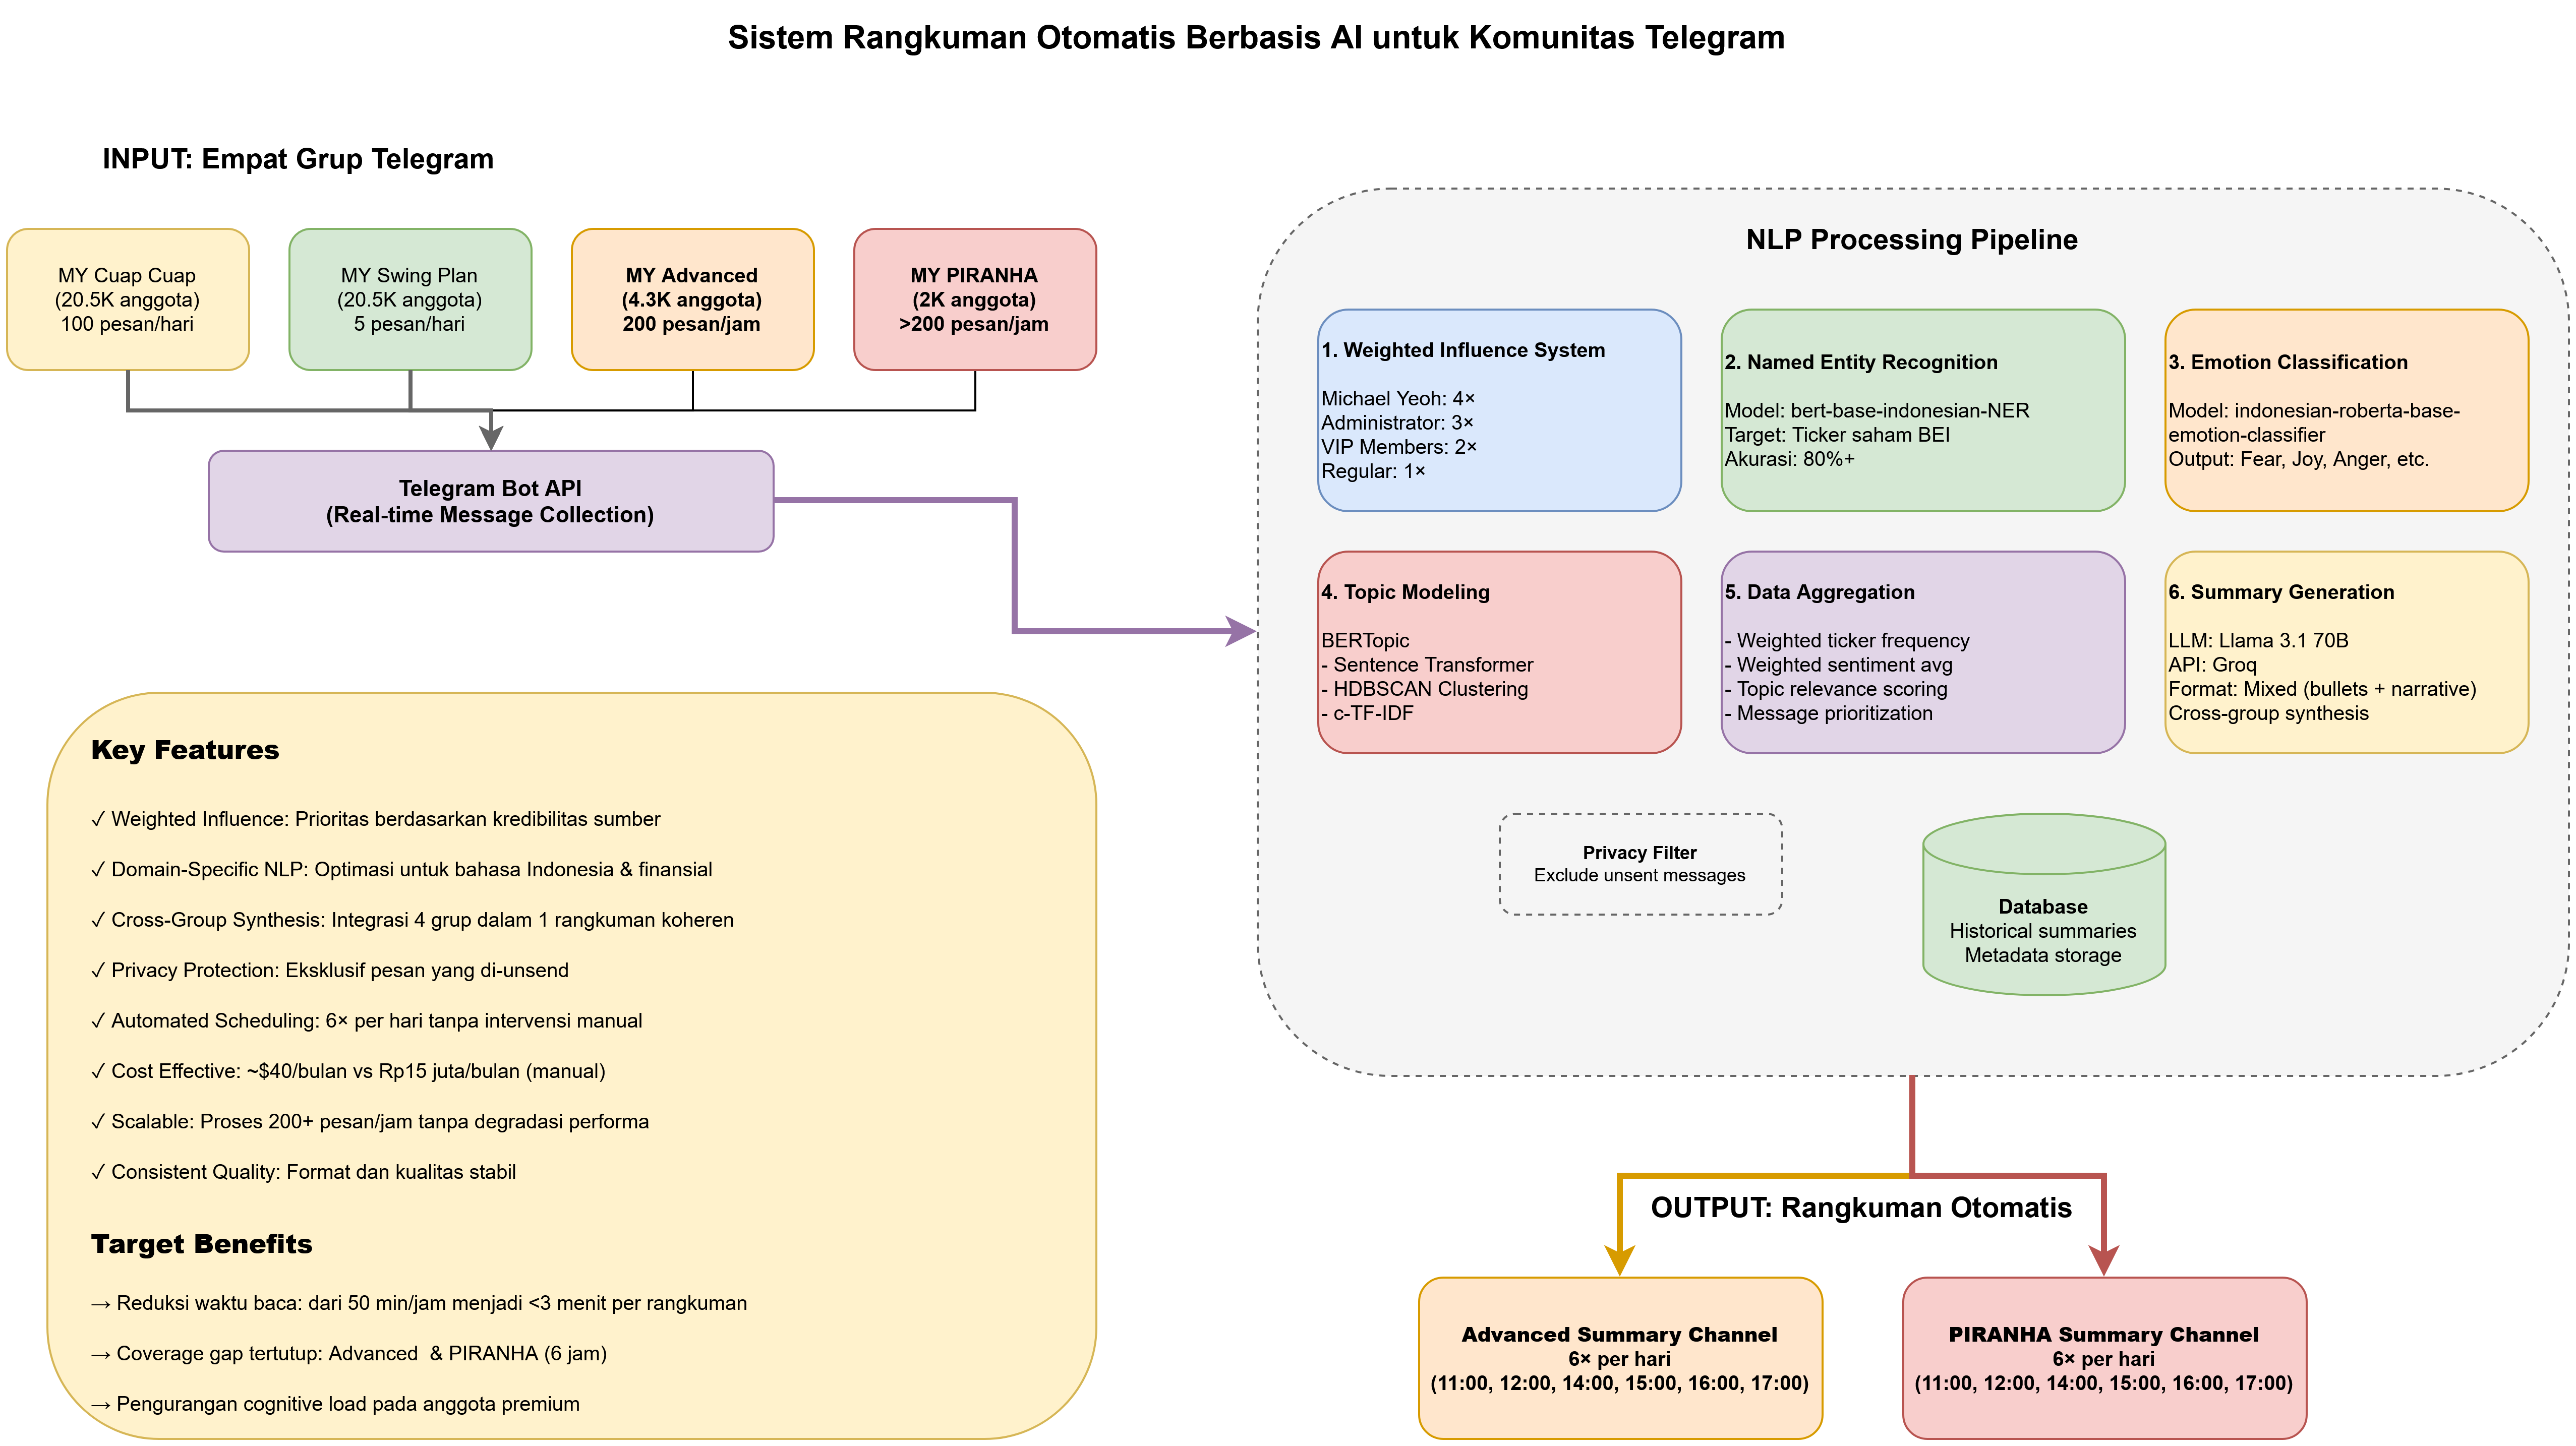
\includegraphics[width=1.0\textwidth]{image/proposed-solution-diagram.png}
  \caption{Arsitektur sistem rangkuman otomatis berbasis AI yang diusulkan dengan \textit{pipeline} NLP terintegrasi, \textit{weighted influence system}, dan sintesis lintas-grup}
  \label{fig:proposed-solution}
\end{figure}

Sistem yang diusulkan mengimplementasikan arsitektur tiga-lapis (\textit{three-tier architecture}) yang terdiri dari:

\begin{enumerate}
\item \textbf{Input Layer:} Empat grup Telegram yang terhubung ke Telegram Bot API untuk pengumpulan pesan \textit{real-time}.

\item \textbf{Processing Layer:} \textit{Pipeline} NLP yang mengintegrasikan enam komponen utama untuk ekstraksi intelijen dan generasi rangkuman.

\item \textbf{Output Layer:} Dua kanal output terpisah untuk Advanced dan PIRANHA yang mengirimkan rangkuman otomatis enam kali per hari.
\end{enumerate}

% ==========================================
\section{Komponen Utama Sistem yang Diusulkan}
\label{sec:system-components}

\subsection{\textit{Weighted Influence System}}

Komponen pertama dan paling kritis adalah sistem bobot pengaruh yang memberikan prioritas berbeda berdasarkan peran pengirim dalam hierarki komunitas:

\begin{itemize}
\item \textbf{Michael Yeoh (Bobot 4×):} Sebagai pemimpin komunitas dan ahli utama, kontribusinya mendapat bobot tertinggi.
\item \textbf{Administrator (Bobot 3×):} Dua administrator dengan kredibilitas tinggi mendapat bobot di atas rata-rata.
\item \textbf{VIP Members (Bobot 2×):} Investor berpengalaman dengan \textit{track record} yang terbukti.
\item \textbf{Regular Members (Bobot 1×):} Anggota standar dengan bobot dasar.
\end{itemize}

Sistem ini memastikan bahwa ticker saham, sentimen, dan topik yang disebutkan oleh sumber kredibel mendapat prioritas lebih tinggi dalam rangkuman, mencerminkan prinsip bahwa "tidak semua opini memiliki bobot yang sama" yang diidentifikasi oleh Si et al. (2014).

\subsection{\textit{Named Entity Recognition} (NER)}

Komponen NER menggunakan model \textit{bert-base-indonesian-NER} untuk mengekstrak entitas finansial dengan fokus pada kode ticker saham yang terdaftar di Bursa Efek Indonesia (BEI). Model ini dikombinasikan dengan \textit{whitelist} ticker BEI untuk memastikan hanya saham valid yang dikenali. Target akurasi minimal 80\% untuk \textit{precision} dan \textit{recall}, dengan validasi menggunakan dataset annotated dari pesan historis komunitas.

\subsection{Klasifikasi Emosi}

Berbeda dengan analisis sentimen biner tradisional, sistem menggunakan \textit{indonesian-roberta-base-emotion-classifier} untuk mendeteksi spektrum emosi yang lebih nuansa termasuk ketakutan (\textit{fear}), kegembiraan (\textit{joy}), dan kemarahan (\textit{anger}). Klasifikasi emosi sangat relevan untuk komunitas finansial karena keputusan investasi ritel dipengaruhi kuat oleh emosi, dan deteksi emosi kolektif dapat mengindikasikan psikologi pasar (misalnya, \textit{fear} tinggi dapat menandakan potensi \textit{panic selling}).

\subsection{\textit{Topic Modeling} dengan BERTopic}

BERTopic digunakan untuk mengidentifikasi topik diskusi dominan dalam setiap periode rangkuman. Metodologi ini dipilih karena superioritas untuk teks pendek dan informal yang telah divalidasi secara empiris (Egger \& Yu, 2022). \textit{Pipeline} BERTopic mencakup:

\begin{enumerate}
\item \textit{Sentence Transformer} untuk menghasilkan \textit{contextual embeddings}
\item HDBSCAN untuk \textit{clustering} adaptif berbasis kepadatan
\item \textit{Class-based TF-IDF} (c-TF-IDF) untuk ekstraksi representasi topik
\end{enumerate}

Parameter \textit{min\_cluster\_size} dioptimalkan untuk volume pesan tinggi (200+ per jam) agar menghasilkan topik yang tidak terlalu granular namun tetap interpretatif.

\subsection{Agregasi Data dengan \textit{Weighted Influence}}

Komponen agregasi mengintegrasikan output dari NER, klasifikasi emosi, dan BERTopic dengan sistem \textit{weighted influence}. Proses agregasi mencakup:

\begin{itemize}
\item \textbf{Frekuensi Ticker Tertimbang:} Ticker yang disebutkan oleh sumber kredibel (bobot tinggi) mendapat skor agregat lebih tinggi.
\item \textbf{Sentimen Emosi Rata-rata Tertimbang:} Emosi diagregasi menggunakan rata-rata tertimbang berdasarkan bobot pengirim.
\item \textbf{Skor Relevansi Topik:} Pesan diprioritaskan berdasarkan relevansi dengan topik dominan yang teridentifikasi.
\item \textbf{Prioritisasi Pesan untuk Konteks LLM:} Subset pesan dengan skor tertinggi dipilih sebagai konteks untuk generasi rangkuman.
\end{itemize}

\subsection{Generasi Rangkuman dengan \textit{Large Language Model}}

Komponen akhir menggunakan Llama 3.1 70B melalui Groq API untuk menghasilkan rangkuman naratif. LLM menerima input terstruktur yang mencakup:

\begin{enumerate}
\item Topik dominan dari BERTopic
\item Ticker teragregasi dengan sentimen tertimbang
\item Subset pesan prioritas dari keempat grup
\item Instruksi eksplisit untuk sintesis lintas-grup
\end{enumerate}

Format output adalah \textit{mixed} yang menggabungkan \textit{bullet points} untuk informasi terstruktur (saham, metrik, sinyal) dengan paragraf naratif untuk konteks dan analisis, mengadaptasi prinsip \textit{multi-granular decoding} dari Chen et al. (2021).

\subsection{Perlindungan Privasi dan Basis Data}

Sistem mengimplementasikan mekanisme perlindungan privasi eksplisit dengan mengecualikan pesan yang telah di-\textit{unsend} oleh pengirim dari pemrosesan. Semua rangkuman historis beserta metadata (timestamp, jumlah pesan diproses, topik terdeteksi) disimpan dalam basis data untuk \textit{audit trail} dan akses retroaktif.

% ==========================================
\section{Aliran Data dan Proses Operasional}
\label{sec:data-flow}

\subsection{Aliran Data \textit{End-to-End}}

Proses operasional sistem dapat dipahami melalui aliran data \textit{end-to-end} berikut:

\begin{enumerate}
\item \textbf{Pengumpulan Pesan (Continuous):} Telegram Bot API terhubung ke empat grup dan mengumpulkan pesan secara \textit{real-time}. Pesan disimpan dalam \textit{buffer} dengan timestamp dan metadata pengirim.

\item \textbf{\textit{Windowing} Temporal (Hourly):} Sistem menggunakan jendela waktu satu jam untuk mengakumulasi pesan. Pada akhir setiap periode (11:00, 12:00, 14:00, 15:00, 16:00, 17:00), \textit{trigger} diaktifkan untuk memulai \textit{pipeline} pemrosesan.

\item \textbf{Pemrosesan Paralel:} Tiga komponen NLP dijalankan secara paralel pada \textit{batch} pesan: (a) NER untuk ekstraksi ticker, (b) Klasifikasi emosi untuk deteksi sentimen psikologis, (c) BERTopic untuk identifikasi topik. Paralelisasi mengurangi latensi total pemrosesan.

\item \textbf{Agregasi dengan \textit{Weighted Influence}:} Output dari ketiga komponen diagregasi dengan menerapkan bobot berdasarkan peran pengirim. Hasil agregasi mencakup ticker tertimbang, emosi rata-rata tertimbang, dan topik dominan.

\item \textbf{Prioritisasi dan Seleksi Konteks:} Pesan diprioritasikan berdasarkan kombinasi skor relevansi topik, bobot pengirim, dan kebaruan informasi. Subset pesan dengan skor tertinggi dipilih untuk dimasukkan dalam konteks LLM (dibatasi oleh \textit{context window} maksimum).

\item \textbf{Generasi Rangkuman:} LLM menghasilkan rangkuman naratif yang mensintesis informasi dari keempat grup. \textit{Prompt engineering} eksplisit menginstruksikan LLM untuk mengidentifikasi hubungan semantik antar informasi dari grup berbeda.

\item \textbf{Distribusi Output:} Rangkuman yang dihasilkan dikirim ke dua kanal output terpisah: satu untuk Advanced, satu untuk PIRANHA. Rangkuman juga disimpan dalam basis data dengan metadata lengkap.
\end{enumerate}

\subsection{Jadwal Operasional}

Sistem beroperasi dengan jadwal tetap yang disesuaikan dengan jam perdagangan saham Indonesia (09:00-16:00):

\begin{itemize}
\item \textbf{11:00:} Rangkuman periode 09:00-11:00 (jam pembukaan + 2 jam pertama)
\item \textbf{12:00:} Rangkuman periode 11:00-12:00 (menjelang istirahat siang)
\item \textbf{14:00:} Rangkuman periode 12:00-14:00 (sesi siang)
\item \textbf{15:00:} Rangkuman periode 14:00-15:00 (menjelang penutupan)
\item \textbf{16:00:} Rangkuman periode 15:00-16:00 (jam penutupan)
\item \textbf{17:00:} Rangkuman periode 16:00-17:00 (analisis \textit{post-market})
\end{itemize}

Jadwal ini memberikan \textit{coverage} komprehensif sepanjang hari perdagangan dengan interval yang cukup sering untuk menangkap dinamika pasar namun tidak terlalu sering hingga menyebabkan \textit{notification fatigue}.

% ==========================================
\section{Perbedaan Kunci dengan Sistem Saat Ini}
\label{sec:key-differences}

Tabel \ref{tab:before-after-comparison} merangkum perbedaan fundamental antara sistem saat ini dan sistem yang diusulkan pada berbagai dimensi kritis.

\begin{longtable}{@{\extracolsep{\fill}} p{4cm} p{5cm} p{5cm}}
\caption{Perbandingan sistem saat ini (\textit{before}) dengan sistem yang diusulkan (\textit{after})}
\label{tab:before-after-comparison} \\
\toprule
\textbf{Aspek} & \textbf{Sistem Saat Ini (Before)} & \textbf{Sistem Diusulkan (After)} \\
\midrule
\endfirsthead

\caption{Perbandingan sistem saat ini dengan sistem yang diusulkan (lanjutan)} \\
\toprule
\textbf{Aspek} & \textbf{Sistem Saat Ini (Before)} & \textbf{Sistem Diusulkan (After)} \\
\midrule
\endhead

\midrule
\multicolumn{3}{r}{\textit{Bersambung ke halaman berikutnya}} \\
\bottomrule
\endfoot

\bottomrule
\endlastfoot

Rangkuman & Manual (hanya Advanced, 1×/hari pukul 10:00); PIRANHA tidak ada & Otomatis (Advanced \& PIRANHA, 6×/hari) \\
\textit{Coverage} & Gap 6 jam (10:00-16:00) untuk Advanced; PIRANHA tidak ada \textit{coverage} & Komprehensif sepanjang jam perdagangan (09:00-17:00) \\
Sintesis Lintas-Grup & Manual oleh anggota yang mengikuti multiple grup & Otomatis melalui \textit{pipeline} NLP terintegrasi \\
Prioritisasi & Tidak ada; semua pesan diperlakukan setara & \textit{Weighted influence} berdasarkan kredibilitas (4×, 3×, 2×, 1×) \\
Ekstraksi Entitas & Manual; bergantung pada kemampuan pembaca & Otomatis dengan NER (target 80\% akurasi) \\
Analisis Sentimen & Tidak ada & Klasifikasi emosi multi-kelas (fear, joy, anger, etc.) \\
Identifikasi Topik & Tidak ada; anggota harus mengidentifikasi sendiri & BERTopic untuk deteksi topik dominan otomatis \\
Konsistensi & Variabel; bergantung pada \textit{curator} yang tersedia & Stabil; format dan kualitas konsisten \\
Biaya Operasional & Rp 15 juta/bulan (3 asisten manual) & \$40/bulan (~Rp 600K) untuk Groq API \\
Skalabilitas & Tidak \textit{scalable}; memerlukan penambahan personel & Tinggi; dapat menangani 250+ pesan/jam tanpa degradasi \\
Waktu Akses Informasi & 50+ menit/jam untuk membaca 200 pesan & Kurang dari 3 menit per rangkuman \\
Perlindungan Privasi & Manual; tidak konsisten & Otomatis; eksklusi pesan yang di-\textit{unsend} \\
\end{longtable}

% ==========================================
\section{Nilai Proposisi dan \textit{Expected Outcomes}}
\label{sec:value-proposition}

Sistem rangkuman otomatis yang diusulkan menawarkan nilai proposisi yang jelas untuk berbagai \textit{stakeholder}:

\subsection{Untuk Anggota PIRANHA (Target Primer)}

\begin{itemize}
\item \textbf{Reduksi Waktu Konsumsi Informasi:} Dari 50+ menit per jam (membaca 200+ pesan) menjadi kurang dari 3 menit per rangkuman—reduksi 94\%.
\item \textbf{Akses Pertama ke Rangkuman:} PIRANHA yang sebelumnya tidak memiliki rangkuman sama sekali kini mendapat enam rangkuman per hari.
\item \textbf{Prioritisasi Otomatis:} Informasi dari Michael Yeoh dan investor berpengalaman diprioritaskan secara algoritmik.
\end{itemize}

\subsection{Untuk Anggota Advanced (Target Sekunder)}

\begin{itemize}
\item \textbf{Penutupan Gap \textit{Coverage}:} Dari satu rangkuman (10:00) menjadi enam rangkuman sepanjang hari.
\item \textbf{Standardisasi Format:} Konsistensi format dan kualitas menggantikan variabilitas rangkuman manual.
\item \textbf{Sintesis Lintas-Grup:} Akses ke insight terintegrasi dari Cuap Cuap, Swing Plan, dan diskusi PIRANHA dalam satu rangkuman.
\end{itemize}

\subsection{Untuk Michael Yeoh dan Administrator}

\begin{itemize}
\item \textbf{Reduksi Beban Manual:} Eliminasi kebutuhan untuk koordinasi pembuatan rangkuman manual.
\item \textbf{\textit{Scalability}:} Sistem dapat melayani pertumbuhan komunitas tanpa penambahan biaya proporsional.
\item \textbf{\textit{Content Strategy Insights}:} Akses ke analisis topik dan sentimen agregat untuk \textit{informed decision-making}.
\end{itemize}

\subsection{\textit{Expected Outcomes}}

Berdasarkan desain sistem dan target metrik non-fungsional yang telah didefinisikan dalam Bab \ref{chap:analisis-masalah}, \textit{expected outcomes} penelitian ini meliputi:

\begin{enumerate}
\item \textbf{Reduksi \textit{Information Overload}:} Penurunan signifikan dalam waktu yang dihabiskan anggota untuk konsumsi informasi, diukur melalui survei sebelum dan sesudah implementasi.

\item \textbf{Peningkatan Efisiensi Akses Informasi:} Anggota dapat mengakses insight penting dalam kurang dari 3 menit per rangkuman versus 50+ menit untuk membaca pesan mentah.

\item \textbf{Reduksi \textit{Cognitive Load}:} Penurunan beban kognitif yang dialami anggota, diukur melalui metrik subjektif seperti \textit{NASA Task Load Index} (NASA-TLX) atau kuesioner \textit{cognitive load} yang disesuaikan.

\item \textbf{Peningkatan \textit{User Satisfaction}:} Kepuasan pengguna terhadap akses informasi dan kualitas rangkuman, diukur melalui \textit{System Usability Scale} (SUS) atau metrik kepuasan kustom.

\item \textbf{Validasi Teknis:} Pencapaian target metrik non-fungsional termasuk akurasi NER 80\%+, \textit{response time} kurang dari 5 menit, dan \textit{system uptime} 95\%+ selama jam perdagangan.
\end{enumerate}

Validasi komprehensif terhadap \textit{expected outcomes} ini akan dilakukan dalam fase \textit{Evaluation} metodologi DSRM yang akan dijalankan sebagai bagian dari implementasi tugas akhir. Metodologi evaluasi detail, termasuk desain eksperimen, metrik, dan instrumen pengukuran, akan dikembangkan lebih lanjut setelah persetujuan proposal ini.
